%%% -*-LaTeX-*-

\chapter{A Visualization Application in Nuclear Engineering}
\label{ch:visualization}
Nuclear fuel performance behavior is a complex and multiphysical phenomenon that is, nonetheless, crucial in determining both the economic and safety performance of a nuclear power plant.
%
Since the 2011 nuclear accident in Fukushima, Japan, significant research has been focused on improving the simulation capability of fuel behavior to design safer (i.e.,\ accident-tolerant) fuel.
%
Qualification of a new fuel design is a long process lasting for years and costing billions of dollars.
%
It is therefore natural to try to improve this process by increasing the understanding of the new fuel design behavior via sensitivity analysis (e.g.,~\cite{IkonenTulkki2014,PastoreSwilerHales2015}) before starting any physical experiment phase.

Given the large span of phenomena impacting fuel performance, engineers are tasked with finding the optimal design in a multidimensional simulation space where the system behavior is potentially nonlinear.
%
Sensitivity analysis via regression has historically been used to guide engineers in the optimization process and in identifying the dominant phenomena.
%
However, using a simple linear regression model in \emph{global} sensitivity analysis may fail to capture intrinsic local behaviors when the system is highly nonlinear.
%
For this reason, we perform \emph{local} sensitivity analysis and visualization of multidimensional nuclear simulation data using partition-based regression models.
%
We use Morse-Smale regression (MSR)~\cite{GerberRubelBremer2011} to identify regions of approximate monotonic behavior within the system response and perform regression and sensitivity analysis locally on these regions.

HDViz~\cite{GerberBremerPascucci2010} uses the same domain partitioning as MSR.
%
Our collaborating scientists have previous exposure to HDViz in risk assessment of nuclear datasets~\cite{MaljovecWangMandelli2013a,MaljovecWangPascucci2013}.
%
The scientists found merit in HDViz's ability to provide a meaningful partitioning amenable to sensitivity analysis (SA); however the complexity of the visual interface made it difficult to isolate the desired local SA information.
%
Therefore, we seek to provide a more targeted representation of the data for performing SA.

Combining domain decomposition with local regression on the analysis side provides us the opportunity to create more targeted and detailed visual encodings than a global approach.
%
Through close interactions with nuclear scientists, the visual encodings are designed with specific requirements in mind, and we aim to keep each view as simple as possible to enhance its usability.
%
We follow the core design study stages~\cite{SedlmairMeyerMunzner2012}--discover, design, implement, and deploy--in this application-driven research.
%
In this work, we use the established Morse-Smale regression~\cite{GerberRubelBremer2011} in the context of sensitivity analysis, together with other common sensitivity metrics, to represent the main drivers within local regions of the model domain.
%
Such a representation leads to a unique set of visualization design requirements that we subsequently address.
%
In this chapter, we report on the iterative process of refining and extending an existing visualization tool, HDViz~\cite{GerberBremerPascucci2010}, to match the needs of nuclear scientists.
%
Furthermore, we report on the successful integration of our framework into the workflow of RAVEN~\cite{RabitiAlfonsiCogliati2015}, a multipurpose risk assessment and uncertainty quantification software in nuclear engineering.

Our system targets structured/unstructured point cloud data of up to tens of dimensions.
%
We validate and reflect on the efficacy of the new design using a three-dimensional dataset from nuclear fuel analysis.
%
Our goal in this analysis is to understand the effects of different fuel parameters on the stress of the fuel cladding.
%
Excessive stress can lead to cracks in the cladding contaminating the plant environment.

\section{Problem Characterization and Abstraction}
\label{sec:currentWorkflow}
We follow the core stages of a design study~\cite{SedlmairMeyerMunzner2012}, namely, discover, design, implement, and deploy, in this application-driven research.
%
During the \emph{discover} stage, we focus on problem characterization and abstraction.
%
We learn the targeted domain of study (in this case, SA for nuclear simulations) through close interactions with nuclear scientists.
%
In this process, we study their \emph{existing work flow} and \emph{design requirements} to better enable knowledge discovery via analysis and visualization.

\subsection{Existing Workflow}
Before designing our visualization solution, we actively engaged nuclear scientists to understand their domain problems and the existing workflow (i.e., their common practices) in SA.
%
As a first approximation, the scientists typically perform a global SA via linear regression or correlation analysis.
%
Point-wise SA is used to estimate gradient information at specific locations via back-of-envelope computation, or a reduced order model (ROM) is constructed from experimental data whereupon statistical information can be collected.
%
The scientists would also manually divide the data domain into subregions that exhibit changes in gradient behavior based on axis-aligned scatterplot projections; then global SA that combines resampling and ROM construction is applied to each manually extracted subregion.

During the discover stage, we helped the nuclear scientists formulate and examine their data analysis and visualization needs through an iterative process.
%
During this phase, we listen to their description of domain problems, characterize and abstract their problems into design requirements, and obtain feedback regarding abstractions for continuous refinement.
%
We identify several challenges in the existing workflow that are summarized into the design requirements described below.

\subsection{Requirement A: Structure-Based Domain Partitioning\\Amenable to Local SA}
As suggested by Gerber et al.~\cite{GerberRubelBremer2011}, we first considered numerous forms of partition-based regression that can be applied for local SA.
%
However, most of these systems are based on greedy, local operations focusing on optimizing some quality metric.
%
Since the task of our collaborators was understanding trends occurring in the data rather than accurately (potentially overfitting) the data, we selected MSR, as it considers the global structure of the data.

In fact, MSR is particularly suited to this task as each partition is assumed monotonic and thus well described by a simple set of simple sensitivity coefficients.
%
In addition, its flexibility and robustness to noise allow it to be used in an exploratory task such as SA.
%
Existing local SA is restricted to be point-wise, and domain partitioning is done manually via a time-consuming process, whereas our proposed SA, built upon MSR, applies automatically and efficiently to partitions at multiple scales.
%
Using HDViz as a starting point (see Figure~\ref{fig:hdviz}), we iteratively defined and redefined new visual design requirements as well as refining existing ones that satisfy the various SA tasks.

\begin{figure}[!b]
  \centering
  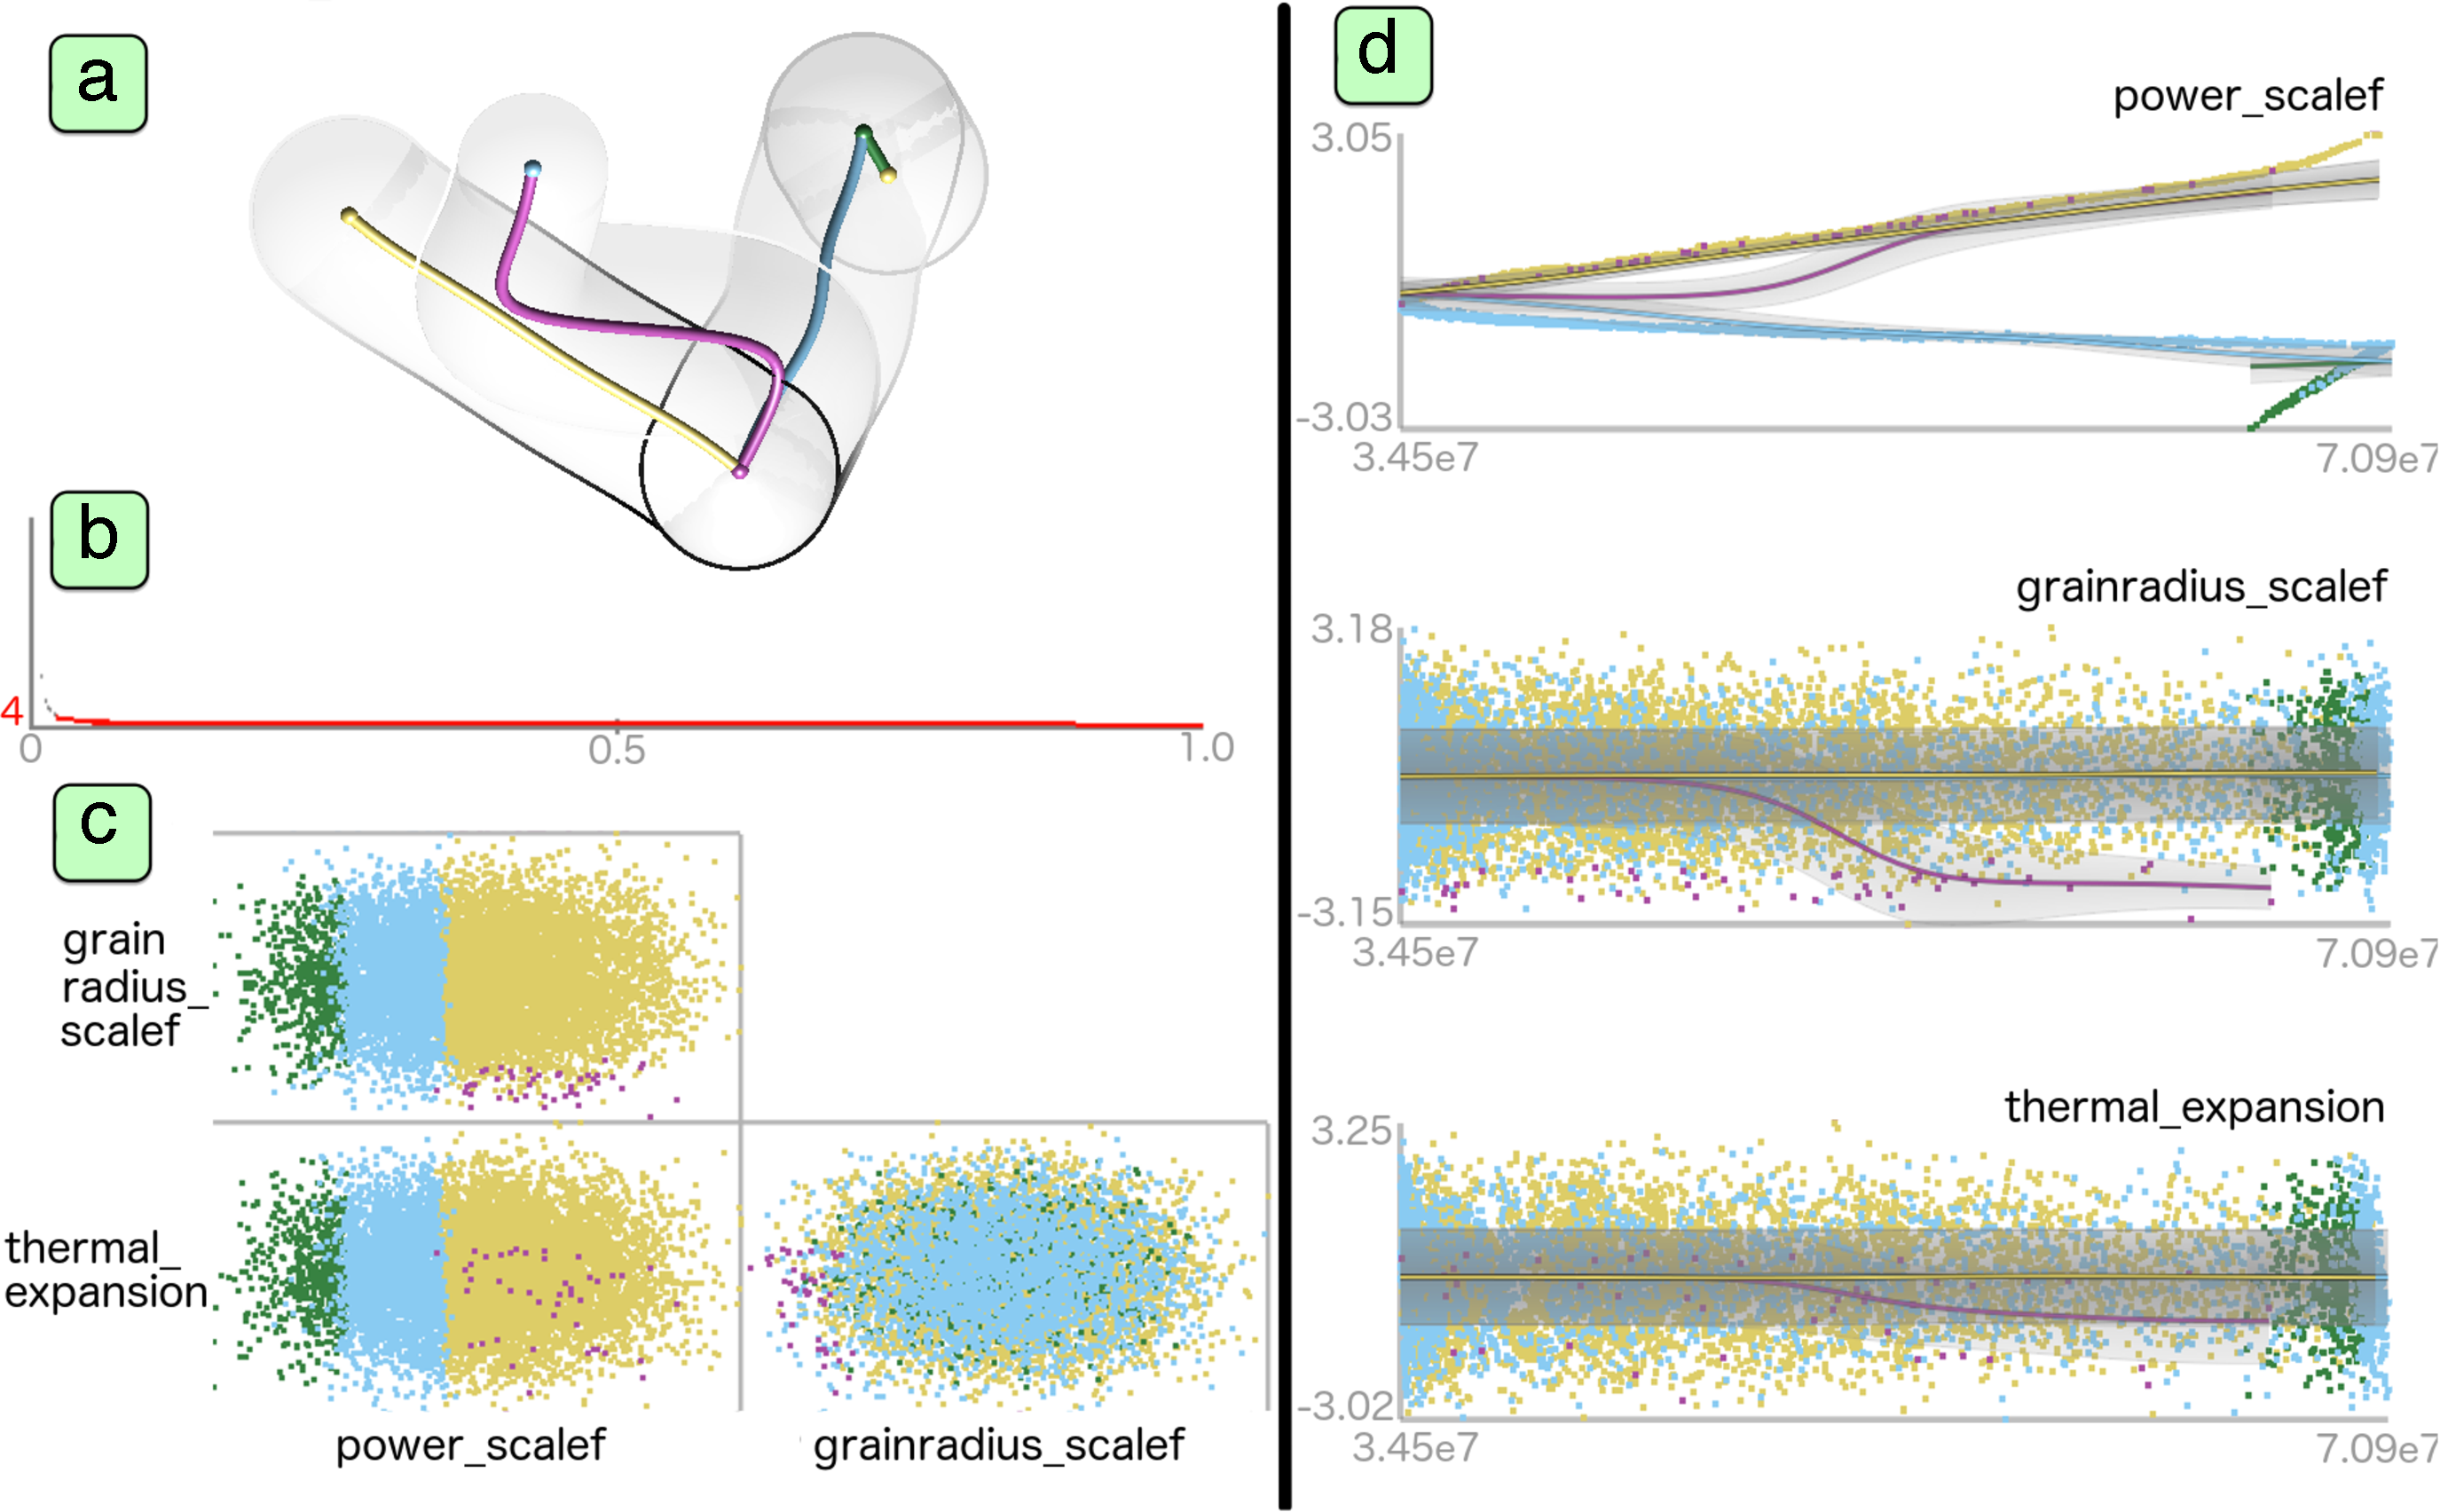
\includegraphics[width=1.0\linewidth]{figs/chap6/HDViz-original}
  \caption[Application of HDViz to nuclear fuel dataset]{HDViz applied to the nuclear fuel
  dataset described in Section~\ref{sec:saApplication}.
  (a) Topological skeleton: each summary curve in the visual space corresponds to a partition of the data; transparent tubes capture the spread (width) and density (luminance) of the partition.
  (b) Persistence chart: number of partitions plotted as a function of scale.
  (c) Scatterplot matrix of partitioned data.
  (d) Inverse coordinate plots: summary curves and partitioned data are projected onto a two-dimensional plot where the x-axis represents the output dimension, and each y-axis
  represents an input dimension. }
  \label{fig:hdviz}
\end{figure}

\subsection{Requirement B: Intuitive Visualization of Data Hierarchy}
Existing visualization using HDViz suffered from three drawbacks for this application.
%
First, it has a very steep learning curve for data practitioners in general.
%
Second, it is particularly nonintuitive for nuclear scientists.
%
And lastly, it has limited support for the SA pipeline.
%
For example, when presented with the topological skeleton seen in Figure~\ref{fig:hdviz}, nuclear scientists questioned the meaning and utility of the oscillations produced by the inverse regression and the geometric interpretation of their two-dimensional projection.
%
During our contextual inquiries~\cite{HoltzblattJones1993}, we noticed that the scientists typically disabled the transparent tubes surrounding the inverse regression curves (Figure~\ref{fig:hdviz}a).
%
Further interactions revealed that the density and geometry information provided was considered ``distracting" and uninformative in their context. Instead, the scientists use the topological tube view to count the number of partitions and extrema at various scales.

Selecting the ``appropriate" scale (i.e., persistence level) from the persistence chart remains an unintuitive process when the scientists are rarely aware of how many ``noisy" features exist in the data. We have invested effort designing various ways to convey such information to the users, as evidenced in Section~\ref{sec:saDesign}.
%
Understanding how the scientists interact with the topological view has greatly influenced its design in our iterative process.
%
We understand that the scientists are primarily interested in a high-level picture of their data; therefore, we simplify our visualization to an abstract two-dimensional representation that enables easier selection and manipulation of partitions and supports well-integrated, interactive selection of scales.
%
Finally, the new visual representations should not only convey information about different scales within the data hierarchy, but also provide context about the
partitions within a fixed scale.
%
The topology map described in Section~\ref{sec:saDesign} is designed to fulfill such requirements.

\subsection{Requirement C: Integration of Common Practices\\with New Designs}

We incorporate visual tools that are familiar to the nuclear scientists (e.g., scatterplots) into our new visual design to ease the knowledge discovery process.
%
For example, the scientists could select a MSC-based partition and observe its associated point cloud clustered in a geometrically coherent space in the corresponding scatterplot.
%
Such an integration gives the users some intuition of how the topological partitioning is being performed.
%
In addition, the scientists find that the scatterplots also provide some sense of data density within each partition -- such information is vital to the users as it is directly related to the confidence associated with the derived sensitivity information.
%
Knowing such details also allows us to encode density information into other representations not prone to the occlusion problem.

\clearpage

\subsection{Requirement D: Presentation of Comparative and\\Quantitative Information}

Initial visualizations of the sensitivity information focus on a comparative analysis that uses shapes of different sizes to convey differences among individual  partitions in the data.
%
Although it is useful for quickly detecting major trends, the scientists have requested the numeric measurements of each partition be displayed as this information is more familiar to them and gives them the increased amount of accuracy necessary for decision-making.
%
Additional designs have been suggested (such as the fitness view detailed in Section~\ref{sec:saDesign}) by the scientists that allow us to better understand their mental model of the data and design our visualization accordingly.

\subsection{Requirement E: Scalable Analysis and Visualization}

The existing SA capabilities do not scale well with the increasing number of parameters/dimensions, but our proposed SA using MSR scales well in high dimensions.
%
Given point cloud data, the analysis in~\cite{GerberRubelBremer2011} has shown that the algorithm in~\cite{GerberBremerPascucci2010} provides a good approximation of the true MSC of the underlying (unknown) function when the smallest feature (signal) of $f$ has a persistence that is at least an order of magnitude larger than the standard deviation of the noise.
%
The running time of the MSC does not depend on the ambient dimension of data points, but rather the topological complexity (e.g., number of local extrema) of the underlying function.
%
Therefore, we employ a typical assumption on our targeted datasets such that they have moderate  topological complexity, and their topological features can be well approximated.
%
In addition, we require that the new visual design remains intuitive and informative even with increasing dimensionality.
%
Scalable visualization is discussed in Section~\ref{sec:topologyMap}.

\section{Visualization Design and Implementation}
\label{sec:saDesign}

In the \emph{design} stage, we focus on data abstraction, visual encoding, and interaction mechanisms~\cite{SedlmairMeyerMunzner2012}.
%
We have proposed multiple visual encodings where the feedback from nuclear scientists helped us narrow them down to a few usable solutions.
%
These solutions were integrated into a linked view system with multiple visual components providing interactive functionalities, as illustrated in Figure~\ref{fig:design-overview}.

\begin{figure}[ht]
  \centering
  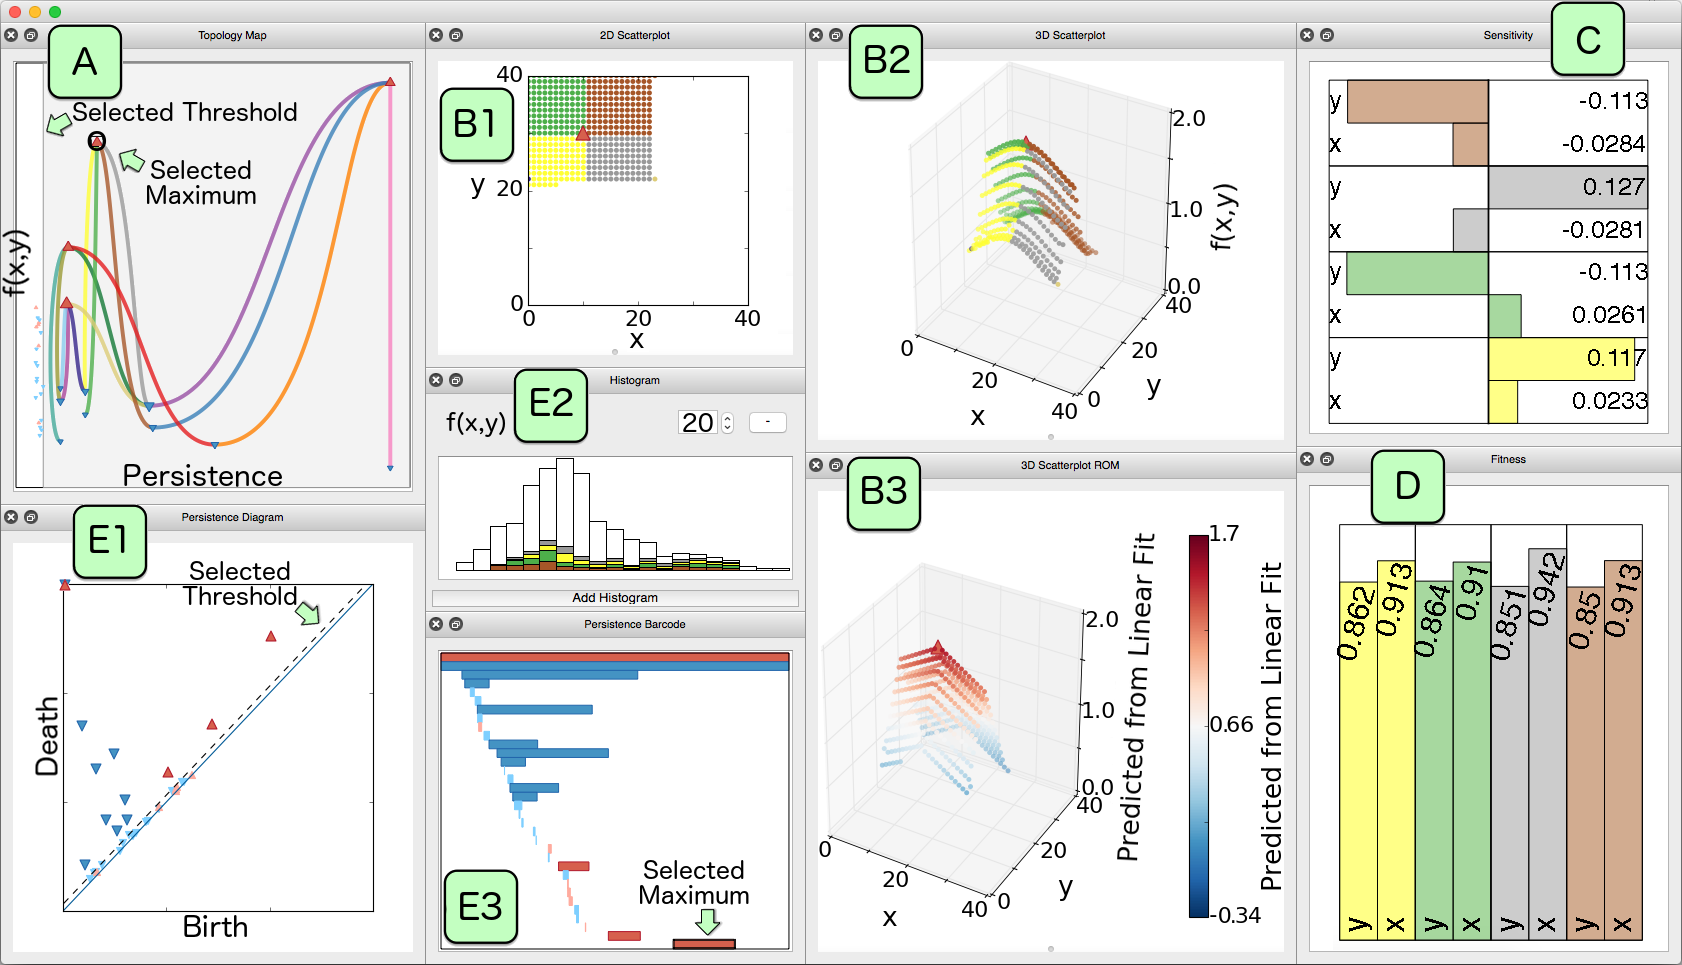
\includegraphics[width=\linewidth]{figs/chap6/design-overview}
  \caption[RAVEN visual interface applied to synthetic data]{Our linked view visualization system using a synthetic two-dimensional test function.
  %
  The system includes (A) topology map, (B1-B3) scatterplots, (C) sensitivity view, (D) fitness view, (E1) persistence diagram, (E2) histogram, and (E3) persistence barcode.
  }
  \label{fig:design-overview}
\end{figure}

A typical workflow begins with the \emph{topology map}, where a user can navigate through partitionings at different scales, and at a chosen scale, explore the structure of the partitions.
%
Within this view, one can understand at a glance the number of local extrema for a given partitioning, their relative importance encoded by persistence, and their connectivity.
%
The appropriate choice of scale is then validated by the \emph{persistence diagram}~\cite{Cohen-SteinerEdelsbrunnerHarer2007} and the \emph{barcode}~\cite{CarlssonZomorodianCollins2004}.
%
At a fixed scale, the user then selects a subset of partitions for further SA.
%
Two-dimensional or three-dimensional scatterplots can be constructed for selected partitions by choosing any two or three input/output dimensions, where the output dimensions include both observed and predicted values.
%
Subsequently, the user can choose to build a \emph{histogram} of any chosen input/output dimension.
%
Such a histogram can also be used for selecting and filtering data for further analysis.
%
Finally, sensitivity information is computed when requested and then visualized on a per dimension basis using the \emph{sensitivity view}, and linear fitness information in terms of $R^2$ score is given in the \emph{fitness view}.
%
We give a detailed description of the \emph{primary} visual encodings below: topology map, scatterplot projection, sensitivity view, and fitness view;  followed by a brief introduction to the \emph{secondary} visual encodings: persistence diagram, barcode, and histograms.

\subsection{Topology Map}
\label{sec:topologyMap}
The topology map is a key data abstraction within our design study.
%
It is a two-dimensional representation of the data that highlights the topological structure of the given data.
%
We generate and validate such an abstraction through an active and cyclic design process with the scientists to arrive at its current form.
%
The topology map encodes the locations of local extrema defined by their persistence and function values, as well as their connectivities (i.e., curves describing flow from a minimum to a maximum).
%
Such a visualization is, in spirit, similar to the topological skeleton proposed in~\cite{GerberBremerPascucci2010} and applied to nuclear probabilistic risk assessment~\cite{MaljovecWangMandelli2013a,MaljovecWangPascucci2013}.
%
However, based on the new requirements outlined in Section~\ref{sec:currentWorkflow}, we have completely redesigned such a visual encoding to provide a topological summary that omits geometric information but  preserves the underlying structure essential to understanding the data partitioning, thereby greatly improving its usability and scalability.

As illustrated in Figure~\ref{fig:design-overview}A, each local extremum is mapped onto a two-dimensional plane, whose \emph{x-axis} represents its \emph{persistence} and the \emph{y-axis} corresponds to its \emph{function value} (i.e., $f(x,y)$).
%
Therefore, local maxima (minima) move toward the top (bottom) of the display, respectively; more robust features appear to the right, whereas noisy ones tend to the left.
%
Encoding function value to the y-axis is well aligned with the scientists' understanding of typical two-dimensional function plots where the dependent variables are mapped to the y-axis; in fact, the inverse coordinate plots used in HDViz (Figure~\ref{fig:hdviz}d) are often misinterpreted for violating this common notion.
%
In addition, the local maxima (minima) are upward (downward) pointing red (blue)  triangles for fast visual differentiation and counting.

Selecting the appropriate scale (i.e., persistence level) for data partitioning is essential during the exploratory process since it helps the user to understand the data hierarchy and sensitivity information.
%
The above design also provides a natural separation between features and noise.
%
The user is able to choose a scale by clicking anywhere in the plot, which creates a vertical line passing through the cursor location, separating the local extrema into those that represent robust topological features (gray region on the right) and those that represent topological noise (white region on the left).
%
Extrema in the gray region are visualized together with their connectivities.
%
Their sizes correspond to the point densities in their surrounding regions.
%
Extrema in the white region are rendered with a default minimum size and therefore do not draw the user's attention away from more salient features but still provide context.

Selection of the scale parameter is an interactive process that is hard to automate, where the user is free to explore and construct ROMs at arbitrary levels.
%
In \emph{persistence simplification}~\cite{Cohen-SteinerEdelsbrunnerHarer2007,EdelsbrunnerLetscherZomorodian2000}, features and noise are assumed to exist on two separable scales, providing a heuristic to choose a scale (vertical line) that is a clear divider between well-separated clusters of extrema.
%
Additional visual cues also help guide such a selection process.
%
For example, in the fitness view, higher $R^2$ scores typically correspond to better local fits of the model at a chosen scale.
%
On the other hand, density information encoded by the sizes of the extrema  influences the interpretation of the $R^2$ score for a given partition, where a high $R^2$ score for a partition with low point density may not be trustworthy.

Closed user feedback loops help us refine our visual encoding of the topological map.
%
For example, the extrema in the gray region are connected via color-coded, user-adjustable, cubic Bezier curves, each of which represents a Morse-Smale cell (i.e., a data partition).
%
Such a representation affords a level of flexibility to counteract visual clutter.
%
Each partition is identified by one of nine colorblind-safe colors~\cite{Tol2012} that is used throughout
the visual interface.
%
The topological map is used as a high-level atlas to orient users in the data exploration process.
%
It enables efficient comparisons among partitions across multiple scales.
%
The user can select local extrema and partitions via its interactive interface for in-depth analysis via the remaining views.
%
We also defer additional geometric information to other views to avoid sensory overload.

In terms of scalability, in practice, with limited number of data points available and the appropriate choice of scales (potentially high-dimensional), nuclear datasets are typically analyzed with less than 10 partitions (e.g.,~\cite{MaljovecLiuWang2015,MaljovecWangMandelli2013a,MaljovecWangPascucci2013}).
%
For datasets with topological complexity that is beyond moderate, we would employ advanced graph drawing techniques such as edge bundling (e.g.,~\cite{CuiZhouQu2008}).

\subsection{Scatterplot Projection}
\label{sec:scatterPlot}
Scatterplot projection is a common tool familiar to the nuclear scientists with whom we interacted.
%
It allows the user to select up to three dimensions to be mapped to spatial coordinates, and a potential fourth dimension to be mapped to a color space.
%
The dimensions of choice include the input parameters, the observed and predicted output parameters, and the residuals of the ROM.
%
The users are therefore provided with detailed spatial information on demand.
%
The two-dimensional height function example in Figure~\ref{fig:design-overview} includes a two-dimensional scatterplot (involving two inputs $x$ and $y$ in B1), a three-dimensional scatterplot (involving $x$, $y$, and an observed output $f(x,y)$ in B2), and a three-dimensional scatterplot for the local ROMs (involving $x$, $y$, and the predicted output).


\subsection{Sensitivity View}
\label{sec:sensitivityView}
We show per dimension coefficients associated with each partition of the data in signed, horizontal bar chart format.
%
The coefficients displayed can be swapped between the linear coefficients, the Pearson correlation coefficients (PEAR), and the Spearman rank correlation coefficients (SPEAR) introduced in Section~\ref{sec:sensitivity}.
%
The user therefore gains first derivative behavior for each selected partition.
%
There are two important pieces of sensitivity information to convey in our visual encoding: the sign and the relative magnitude of the different coefficients.
%
Using signed bar charts, this information becomes available at a glance, and the ubiquity of bar charts ensures their universal interpretation.
%
These bar charts are grouped by partition for easy comparison, but can also be changed to group by dimension if needed for a specific comparison.

\subsection{Fitness View}
\label{sec:fitnessView}
For each partition, the fitness view reports the fit accuracy as well as its incremental improvement by increasing the dimensionality of the fit.
%
Based on the linear coefficients described in the sensitivity view, the dimensions are ordered by their magnitude and visualized via vertical bar charts.
%
Based on this sorted order of dimensions as a heuristic, we build lower-dimensional linear fits beginning with only the dimension with the largest coefficient in magnitude.
%
We then iteratively add one dimension at a time and recompute an updated linear model.
%
For an $m$-dimensional dataset, we will end up with $m$ different linear fits and for each fit, we compute the coefficient of determination $R^2$ given in Equation~\ref{eq:r_squared}:
%
\begin{equation}
    R^2 = 1 - \frac{\sum_{i=1}^n ( y_i - \hat{y}_i)^2}{\sum_{i=1}^n ( y_i - \bar{y})^2}
    \label{eq:r_squared}
\end{equation}
%
where $n$ is the number of data points and, for the $i$-th data point, $y_i$ is the observed response value, $\hat{y}_i = \mathbf{x_{i}}\boldsymbol\beta$ is the fitted response value, and $\bar{y} = \frac{1}{n}\sum_{i=1}^{n}y_i$ is the mean of the observed response values.

The use of vertical bar charts conveys the stepwise improvement of adding a dimension to the regression model.
%
Typically (but not always), the largest changes in $R^2$ score occur at the beginning, and we are interested to know at what point the value added by increasing the dimensionality becomes negligible, signifying potentially extraneous dimensions.

\subsection{Secondary Visual Encodings}
\label{sec:otherViews}
We include a few secondary visual encodings to enhance and validate insights obtained from the primary ones.
%
The persistence diagram is the classic tool in the form of a two-dimensional scatterplot used for separating signal from noise~\cite{EdelsbrunnerHarer2008}.
%
In a nutshell, a point in the persistence diagram corresponds to a topological feature represented by the pairing of two critical points.
%
The \emph{persistence} of a point (and its corresponding feature) in the diagram is  its distance to the diagonal.
%
When selecting an appropriate scale for partition-based SA, the chosen vertical line in the topology map corresponds to a dotted line in the persistence diagram; a large separation between clusters of extrema in the topology map corresponds to a large separation between clusters of points in the persistence diagram.

The persistence diagram provides a standard and less cluttered view of the distribution of topological features in the data, and offers a complementary and validating alternative when selecting the appropriate scale.
%
In addition, we also include a persistence
barcode (see~\cite{CarlssonZomorodianCollins2004} for details) that encodes similar information as the persistence diagram as another alternative for visual comparison.
%
Histograms are provided on demand and allow the user to visualize the distribution of inputs, outputs, and various computed values on a per partition basis.
%
The histograms also provide an interactive filtering system.
%
These alternative visual encodings are included as part of our parallel prototyping stage, and they are implemented in our final tool to offer diversity and increase efficacy.

\subsection{Implementation Details}

During the \emph{implement} stage of our design study, we carefully choose algorithms, techniques, and programming languages to meet the design requirements of the nuclear scientists, addressing issues such as scalability and usability.
%
Our implementation is integrated into RAVEN, an uncertainty quantification and probabilistic risk assessment tool actively being developed by and for nuclear scientists.
%
This integration creates a platform with good exposure for the new workflow being adopted by the scientists.
%
Close user interactions help us refine our design and implementation in an iterative process.
%
RAVEN is written in Python with a collection of C++ bindings for back-end algorithms.
%
The approximate MSC computation and our version of MSR are implemented in C++, and the graphical interface is implemented using the PySide binding of Qt.
%
Such a programming environment supports rapid software prototyping and ensures tight integration with the existing RAVEN Python code.
%
In addition, our modular implementation and linked view design~\cite{Roberts2007}  are also suitable for extending and expanding the visualization capabilities of RAVEN in the future.

\section{Deployment and Evaluation: Nuclear Fuel Design}
\label{sec:saApplication}
The final \emph{deploy} stage of our design study involves software release and evaluation.
%
To evaluate the efficacy of our design and to gather feedback from the users, our framework is applied to an actual simulation being studied by the scientists involving nuclear fuel performance.
%
As described in Section~\ref{sec:currentWorkflow}, the deployment is tightly integrated into the design stage as a feedback loop, allowing both the user and the designer to exchange ideas on the data and the design.
%
We recount such an iterative process below.

\subsection{Data From Nuclear Fuel Analysis}
\label{sec:applicationBackground}
We consider an analysis of a nuclear fuel rodlet simulation performed using the BISON software~\cite{HalesNovasconePastore2013}, a modern finite-element-based nuclear fuel performance code.
%
The rodlet is axisymmetric and composed of 10 stacked UO$_2$ pellets surrounded by a zirconium alloy shield known as the cladding.
%
We track the midplane von Mises stress occurring on the three-dimensional cladding.
%
High stress can cause the cladding to crack and allow radioactive gas to leak into the plant environment.
%
The simulation looks at a ramping of the linear power in the reactor from time $t=0$, up to $t=10,000$ (seconds), whereupon the power level maintains a constant value for the remainder of the simulation.
%
At $t=0$, the linear power begins at $0$ W/m and then linearly climbs to a value of $25,000$ W/m before leveling off.

The goal is to gain a better understanding of the physics happening at the \emph{contact point} that occurs when the fuel rodlet expands to the point of touching the cladding.
%
The stress on the cladding at $t=0$ is due to a compressive force from the water pressure outside the cladding.
%
As fission occurs, the fuel rod expands as it is heated due to thermal expansion and swelling from the release of fission gas within the microstructure of the fuel.
%
Once contact is made, thermal expansion (of the cladding) exerts a force that counteracts the compressive force from the water pressure, and therefore the stress in the cladding decreases until these forces reach an equilibrium.
%
After the equilibrium point, the expansive forces on the cladding become dominant, causing stress on the cladding as it expands.

In the above scenario, contact is not indicative of a failure state, and is actually expected in these types of environments.
%
The described problems arise only when the stress in the cladding becomes too high.
%
For this study, the scientists vary three input parameters during the simulation: (1) the linear power scaling factor ($\powerf$), a multiplier for the previously described ramping linear power; (2) the grain radius scaling factor ($\grainf$), a multiplier for the size of microstructure elements known as the grains and related to the swelling caused by the fission gas; and (3) the thermal expansion coefficient for the fuel rodlet ($\thermal$), which dictates how quickly the rod expands and thus how quickly it contacts the cladding.
%
The output parameter of interest is the final midplane von Mises stress $\maxs$ (a scalar quantity derived from the Cauchy stress tensor useful in determining at what point the cladding may yield/crack) recorded after a simulation time of $t=10^6$ seconds.
%
All parameters are scaled using z-score standardization to align with both domain and algorithmic practices.

\subsection{Anomaly Detection in an Initial Dataset}
\label{sec:anomaly}

\begin{figure}[htbp]
  \centering
  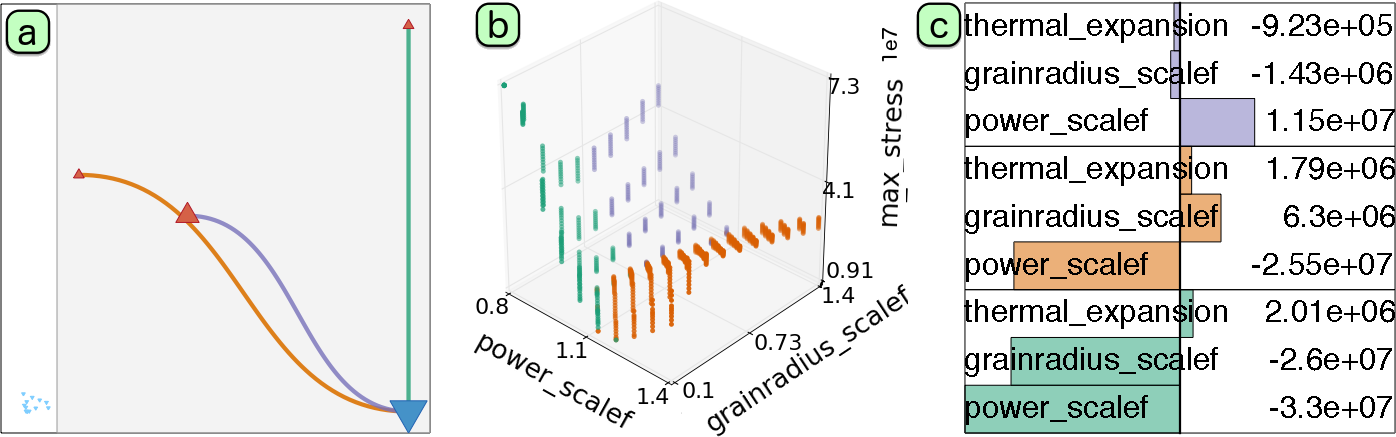
\includegraphics[width=1.0\linewidth]{figs/chap6/bisonError2}
  \caption[Structured sensitivity analysis revealing anomaly in nuclear fuel data]{SA for the initial nuclear fuel dataset.
  (a) Topological map used to separate signal from noise.
  (b) Three-dimensional scatterplot projecting the data onto the two most significant inputs, textbf{power\_scalef} and \textbf{grainradius\_scalef}, with the third dimension reserved for the output, \textbf{midplane\_stress}.
  (c) The linear coefficients of each partition. Note, these results violated the domain scientists' assumption of the data and allowed us to quickly identify an error in the simulation.}
  \label{fig:bisonError}
\end{figure}

Exploration begins with an initial dataset sampled from a
uniform $10\times10\times10$ grid of the parameter space.
%
During the exploration process illustrated in Figure~\ref{fig:bisonError}, the scientists notice an unexpected behavior within the sensitivity view.
%
An increase in the $\thermal$ of the fuel is expected to cause the fuel to expand more rapidly and come into contact with the cladding sooner.
%
The result would cause everything to precipitate faster: a simulation reaching the equilibrium point leads to a higher stress in the cladding; a simulation ending before reaching the equilibrium point (exhibited via lower values of $\powerf$) results in a lower stress.
%
The expectation is that the higher the $\thermal$ is, the higher the stress becomes.
%
However, the linear coefficients for $\thermal$ across partitions in the sensitivity view contradict such an expectation:
(1) $\thermal$ is positive for the green and orange partitions when $\powerf$ is low, and increases when approaching the equilibrium (located at the intersection of the three partitions);
(2) $\thermal$ is negative for the violet partition when $\powerf$ is high, and decreases past the equilibrium.
PEAR and SPEAR coefficients (not shown here) exhibit similar behaviors.

After further investigation with the fuel experts, simulation parameters, aside from the three sampled, were found to be improperly initialized, leading to this anomaly in the initial dataset.
%
This is a very important observation because this particular dataset is being used by multiple ongoing projects where its validity is crucial to their success.
%
% Furthermore, the input files to these simulations are very large and it is not feasible to do a manual check of every simulation parameter setting.
%
Such an anomaly in the dataset itself would not have been exposed via a global SA, since the problem was detected by comparing the behavior of an input parameter from one partition to another where the partitions carry actual physical meaning.

\subsection{Workflow with Corrected Data}
\label{sec:workflow}
After fixing the bug associated with the simulation input, a new dataset is generated for SA from $9517$ simulations using Monte Carlo sampling of the three input dimensions from independent distributions.
%
Starting with the topology map in Figure~\ref{fig:bison}a, a large horizontal gap between two clusters of extrema signifies clear separation between signal and noise in the data.
%
The scientists therefore select a scale (a vertical line) that preserves the three extrema in the gray region as topological features, resulting in two partitions of the data domain.
%
Such a selection is also supported by observing a large gap between two clusters of points within the persistence diagram (Figure~\ref{fig:bison}b), where one cluster contains points near the diagonal $y=x$ and the other contains points far away from the diagonal.
%
As a first-order approximation, the scientists build local linear regression models for these two partitions.

\begin{figure}[b]
  \centering
  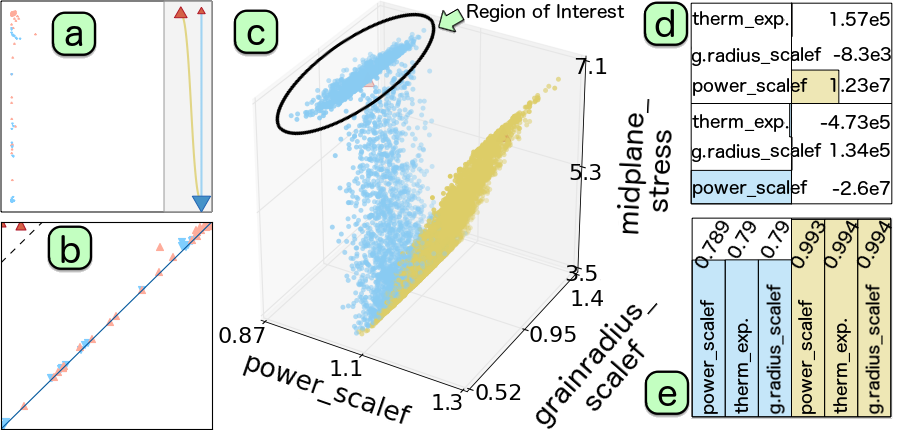
\includegraphics[width=\textwidth]{figs/chap6/bison2}
  \caption[Coarse structured sensitivity analysis on corrected nuclear fuel data]{SA of the new nuclear fuel dataset:
  (a) topology map, (b) persistence diagram, (c) linked scatter plot projection,  (d) linear coefficients, and (e) fitness view with stepwise $R^2$ scores.
  }
  \label{fig:bison}
\end{figure}

The resulting linear coefficients are shown in Figure~\ref{fig:bison}d where the $\powerf$ dominates the behavior of the $\maxs$.
%
Furthermore, the fitness view (Figure~\ref{fig:bison}e) demonstrates that little to no information is gained by incorporating the remaining two dimensions, in either partition of the data.
%
The fitness view also shows that the blue partition is not well described by a linear fit of any number of dimensions (i.e., with all three $R^2$ scores valued roughly at $0.79$).
%
The scientists investigate further by projecting the data onto a scatterplot (Figure~\ref{fig:bison}c) that includes the most sensitive input dimension ($\powerf$) and the output dimension ($\maxs$).
%
From this scatterplot, they detect the nonmonotonic behavior of a region of interest (ROI) within the blue partition, which has low $\powerf$ and high $\maxs$.
%
The scientists then focus on a more refined analysis at a finer scale to try to capture the behavior of the ROI within its own partition.

Figure~\ref{fig:bisonRefined} shows the results after decomposing the domain into three and four partitions at finer scales.
%
The scientists, guided by both the topology map and the scatterplot view, iteratively choose finer and finer scales until the ROI separates itself from the larger blue partition.
%
The first level of refinement produces three partitions in the data (Figure~\ref{fig:bisonRefined}a).
%
Compared to the approximation with two partitions (Figure~\ref{fig:bison}c), the newly constructed magenta partition has relatively low point density (as shown in Figure~\ref{fig:bisonRefined}b) and does not correspond to the ROI.
%
Under the second level of refinement (Figure~\ref{fig:bisonRefined}c), the ROI forms its own partition in green, as illustrated in Figure~\ref{fig:bisonRefined}d.
%
In addition, there is significant improvement in the fitness for the blue region.
%
That is, the three $R^2$ scores increase from roughly $0.790$ to $0.898$ (Figure~\ref{fig:bisonRefined_sensitivity}).
%
Therefore, extracting the desired ROI requires two additional levels of refinements.

\begin{figure}[b]
  \centering
  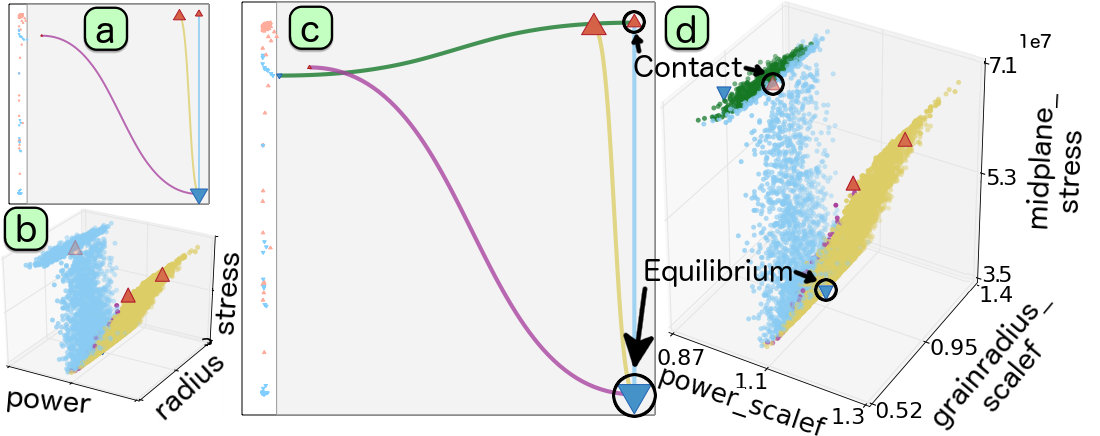
\includegraphics[width=\linewidth]{figs/chap6/bisonRefined3}
  \caption[Refined structured sensitivity analysis on corrected nuclear fuel data]{
  SA of the new nuclear fuel dataset under two refined settings:
  topology maps and scatterplots with three partitions (a)-(b) and four partitions (c)-(d), respectively.}
  \label{fig:bisonRefined}
\end{figure}

\begin{figure}[t]
  \centering
  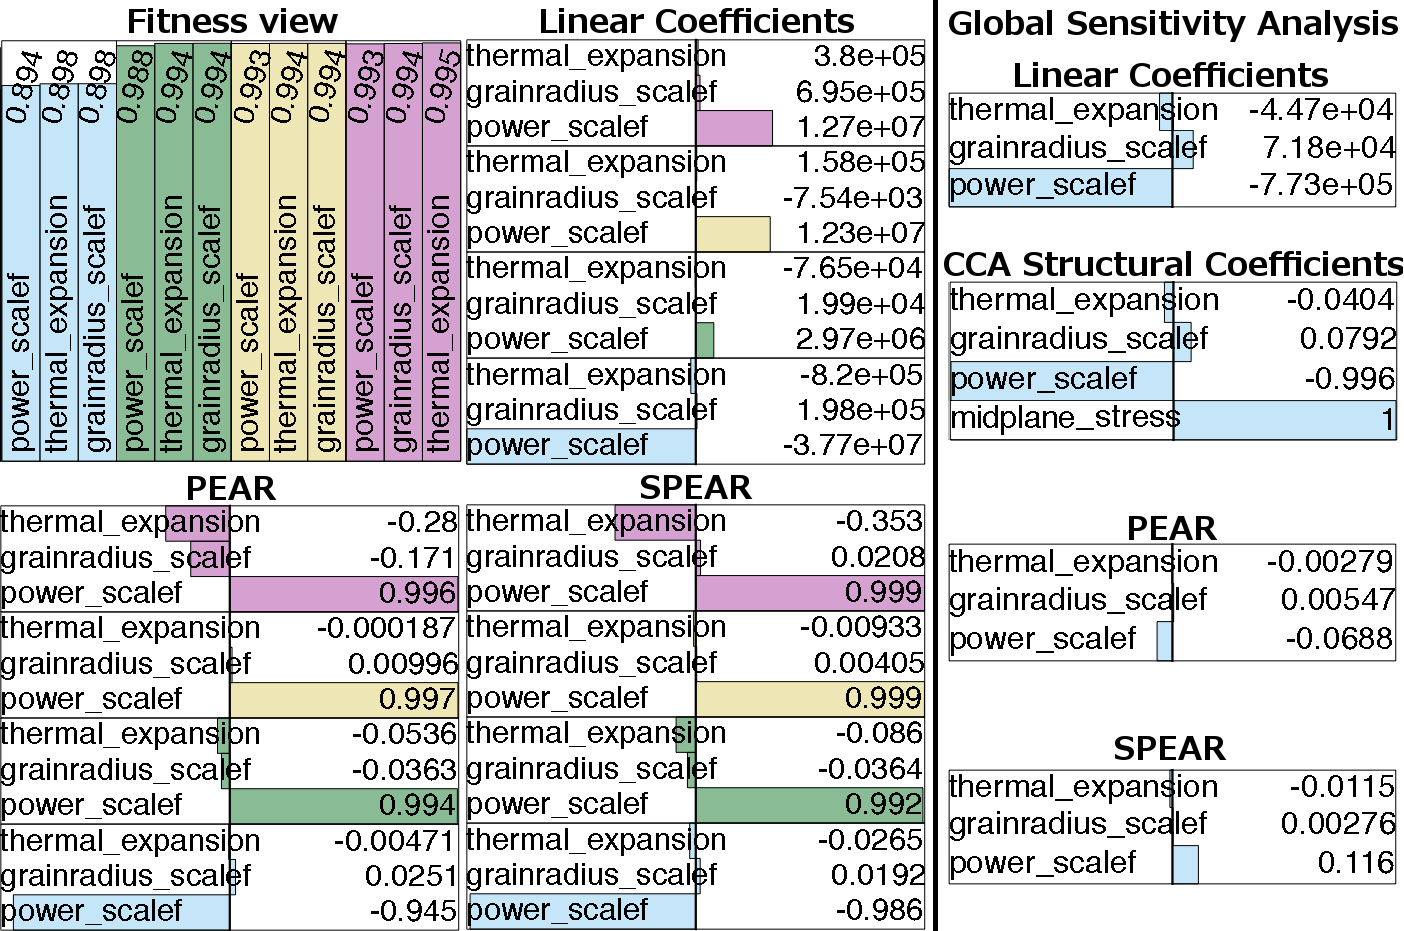
\includegraphics[width=\textwidth]{figs/chap6/bisonRefinedSensitivity2}
  \caption[Comparison of structured sensitivity coefficients versus global coefficients]{
  Left: sensitivity information of the new nuclear fuel dataset under the refined setting with four partitions.
  Right: global SA of the same dataset.
  }
  \label{fig:bisonRefined_sensitivity}
\end{figure}

Under the refined setting with four partitions, the scientists are able to obtain insights that are aligned with their expectation and domain knowledge.
%
Using topology-based domain partitioning allows them to decompose the domain in a physically meaningful way.
%
In particular, the four partitions within the data domain are shown to correspond to various stages of the simulation.
%
The scientists focus on examining the characteristics of each partition and how the partitions interface with one another.
%
First, the interface between the green and blue partitions represents the \emph{contact} point where the fuel touches the cladding (Figure~\ref{fig:bisonRefined}d).
%
Within the green partition (which has very low $\powerf$ values), the net pressure acting on the cladding originates from the external water pressure.
%
Second, the interface between the blue and the combined magenta and gold partitions corresponds to the \emph{equilibrium} point.
%
The blue partition represents the simulations where the expansive forces of the cladding begin to counteract the compressive water pressure force.
%
Within the blue partition, as $\maxs$ decreases and $\powerf$ increases, the simulation moves closer to the equilibrium.
%
Finally, the remaining two partitions (gold and magenta) contain scenarios after the equilibrium point between compressive and expansive stresses, and therefore within these partitions, an increase in $\powerf$ leads to an increase in the dominating expansive stress (i.e., $\maxs$).
%
In terms of sensitivity information (Figure~\ref{fig:bisonRefined_sensitivity} left), $\powerf$ has a strong positive effect on $\maxs$ across the partitions with the exception of the blue region, where it is strongly negative.

Finally, the scientists compare the results from the partition-based local SA (Figure~\ref{fig:bisonRefined_sensitivity} left) with that of a global SA (Figure~\ref{fig:bisonRefined_sensitivity} right).
%
For the global SA, the linear coefficients and CCA structural coefficients~\cite{CrossnoSheadSielicki2015} are used to identify $\powerf$ as the most sensitive parameter, yet its sign heavily depends on the amount of data on either side of the contact and equilibrium points.
%
Similarly, the nonmonotonic global behavior masks the sensitivity associated with $\powerf$ for both PEAR and SPEAR coefficients.
%
On the other hand, the topology-inspired, partition-based SA is able to capture three distinct behaviors in the data, and it highlights the high sensitivity associated with $\powerf$ within each partition.

Using our framework, the scientists have validated the behaviors of a nuclear fuel simulation to be well aligned with their expectations.
%
They are actively investigating higher-dimensional problems where topological partitioning could offer them additional insights that are not readily available via traditional visualization such as scatterplot projections.
%
Our objective in validation has been confirmed by the scientists where they could perform SA faster and with higher accuracy.
%
Our framework also offers a new paradigm in rethinking about SA via topology in nuclear engineering.

\section{Conclusion}
According to our collaborating scientists, our software is the \emph{first} screening tool to enable understanding the dominant impacts of the uncertain parameters with respect to design figures of merit (e.g.,\ internal pressure, stress, etc.).
%
They also found it useful for ranking the uncertain parameters and for the construction of effective and powerful ROMs for an extensive UQ study.
%
Finally, we demonstrated how our tool was able to quickly and effectively highlight anomalous results at the earliest stages of the fuel design process.

The following summary was provided by a collaborating scientist: Recent studies~\cite{BouloreStruzikGaudier2012,IkonenTulkki2014,PastoreSwilerHales2015} have demonstrated the application of SA to the modeling of nuclear fuel behavior, where the considered scenarios have covered both steady-state and transient irradiation and different burnup levels.
%
However, existing results have been presented in terms of output range given the whole input domain (i.e.,\ global SA).
%
Instead, the presented technique allows fuel designers to decompose the analysis into partitions based on actual regimes of fuel behavior (e.g., open fuel-cladding gap or fuel-cladding contact).
%
Fuel performance during these different regimes can be driven by different aspects (e.g., rod fill gas pressure or fuel-cladding contact pressure), and hence, such physically based decomposition may offer more meaningful insight into the specific situations targeted by the analysis.
%
Although designed specifically for nuclear engineers to use, this tool has also been successfully applied to the study of hydrology data where the goal was to understand the global warming potential of various factors involved in implementing a rainwater harvesting system for controlling combined sewer overflows~\cite{Tavakol-Davani2016}.

% \section{Exploration of Limit Surface Probabilities in RISMC Applications}
%   in progress

% \bibliography{\jobname}